\documentclass{article}
\usepackage[utf8]{inputenc}
\usepackage[spanish]{babel}
\usepackage{listings}
\usepackage{graphicx}
\graphicspath{ {images/} }
\usepackage{cite}

\begin{document}

\begin{titlepage}
    \begin{center}
            
        \Huge
        \textbf{Diseño y planeación}
        \LARGE
        \vspace{0.8cm}
        
        Realizado por:\\    
        \textbf{Daniel Ovany Mesa López}\\
        \textbf{Mateo Muñoz Arroyave}
        \vfill
        
        \begin{figure}[htp]
            \centering
            
\includegraphics[width=8cm]{images/EscudoUdeA.png}
        \end{figure}
        
            
        \vspace{0.2cm}
            
        \Large
        Despartamento de Ingeniería Electrónica y Telecomunicaciones\\
        Universidad de Antioquia\\
        Medellín\\
        Octubre de 2021
            
    \end{center}
\end{titlepage}

\tableofcontents

\section{Sección introductoria}\label{intro}
La actividad que realizaremos es un juego donde utilizaremos todo lo aprendido y enseñado por los profesores en clase de informatica, utilizaremos qt y un control de versiones como github para llevar un orden en nuestro proceso del proyecto. El videojuego que se pretende desarrollar es de tipo arcade, este tendrá tres niveles con diferente dificultad, rol multijugador, controles de mando, etc. Con esto buscamos que el usuario emplee una jugabilidad muy analítica para lograr finalizar el juego. En dicho entorno de programación se crearán las respectivas clases y objetos para tener una buena estructuración del diseño del juego.


\section{Sección de contenido} \label{contenido}
Es un juego de escritorio para el pc donde consta de un persojane militar que requiere de un arma para ir acabando con los enemigos que se cruzan en el camino o mas bien van saliendo ovnis y seres extraterrestes, salen en diferentes movimientos y la idea es llegar acabar con ellos y no dejar que ellos te quiten toda la vida, el personaje tiene diferentes armas que disparan con diferentes movimientos tambien adecuandose al movimientos con el que salgan los enemigos, la dificutad del juego se vera reflejado en la velocidad de los enemigos y en la continuidad en la que van saliendo, también en que el personaje tendrá menos balas para derrotarlos, tendremos una tabla de score donde se veran reflejados los mejores puntajes obtenidos. A medida que desarrollamos este proyecto iremos mejorando las idea y el contenido del juego para que sea mas didáctico.

\section{Escenas del juego} \label{contenido}
El juego constará de dos escenas perfectamente diseñadas para soportar el mismo desarrollo en una y en la otra, el usuario antes de iniciar con el juego y al elegir el metodo tiene adicionalmente la opción de escoger el tema de la escena donde se va a jugar, estos cambios de escena sólo serán elegidos por el usuario antes de empezar la partida. En las escenas el jugador contará con una barra de vitalidad, tres tipos de balas diferentes, cantidad diferente de enemigos, cajas de ayuda para el jugador, puntos por enemigo muerto, a medida que transcurre el tiempo el jugador aumenta su score, etc.

\section{Personajes} \label{contenido}
\subsection{Militar} \label{contenido}
El personaje militar es el personaje principal y con el que vamos a tener mas interacción ya que es el que vamos a manipular con mayor frecuencia para combatir contra los enemigos, este personaje se manipula mayor mente con el mouse haciendo click ya que asi podemos señalar la bala que queremos utilizar para el enemigo y poder cambiarla a la hora que lo deseemos, adicionalmente asi mismo podemos señalar con el mouse donde queremos que el personale o el militar dispare la bala y hacia donde dispararla.

\subsection{Ovnis} \label{contenido}
Los ovnis es otro de los personajes principales ya que es el personaje que va a estar interactuando con el personaje militar, pues estos ovnis van saliendo en un ataque desde un extremo de la escena en diferentes movimientos, donde al aumentar su dificultad su cantidad y velocidad de ovnis va a ser mucho mayor asi se vera reflejada la dificultad del juego, al destruir estos ovnis se vera reflejado cierto puntaje que dara cada asesinato de ellos. 

\section{Multijugador} \label{contenido}
En la sección de multijugador tendremos la interaccion de los dos participantes, donde uno controla al militar y el otro controla la salida de los ovnis. El jugador 1 controla al militar desde el mouse donde puede recurrir al cambio de armas y a definir el punto donde quiere la bala, el jugador 2 consta de el control de los ovnis ya que este con el teclado puede controlar a los ovnis que tan frecuentes pueden salir y asi darle la dificultad que desee el jugador, luego se hara un cambio de papales donde le jugador 1 pasara a ser el que controla los ovnis y el jugador 2 a ser el militar, y asi se podra definir el ganador con el mayor puntaje obtenido al final.

\section{Conograma} \label{contenido}

\begin{figure}[htp]
            \centering
            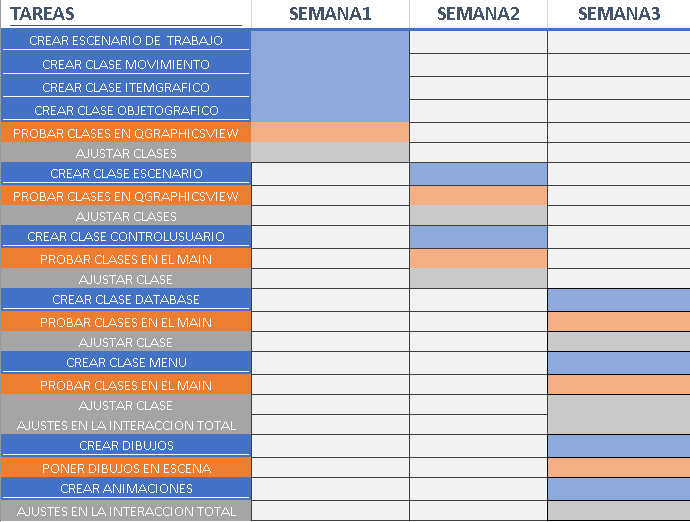
\includegraphics[width=10cm]{images/Cronograma.png}
        \end{figure}

\end{document}
